\documentclass[margin=1pt]{standalone}

\usepackage{tikz}

\usetikzlibrary{
  calc,
  arrows, arrows.meta,
  decorations.pathreplacing,
  calligraphy,
}

\begin{document}
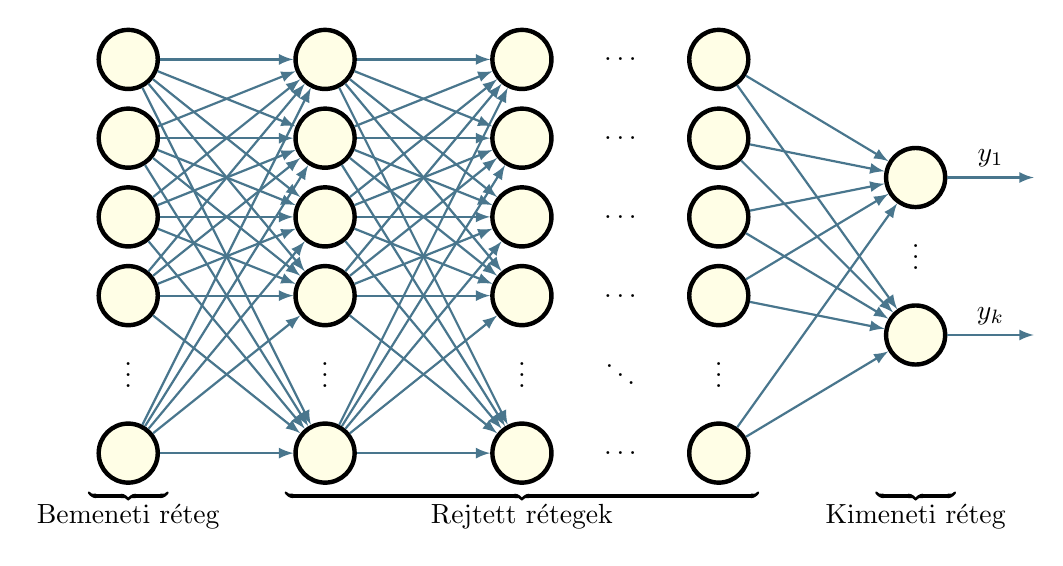
\begin{tikzpicture}[
    ultra thick,
    arr/.style={thick, cyan!50!black},
    lab/.style={font=\ttfamily, black},
    circ/.style={fill=yellow!10, draw=black, circle, minimum size=7.5mm},
  ]
  \foreach \i in {0,1,2,3} {
      \foreach \j in {0,1,2,3,5}{
          \node[circ] (w\i\j) at (2.5*\i,-\j) {};
        }
      \node at (2.5*\i, -3.9) {$\vdots$};
    }
  \node[circ] (w40) at (10, -1.5) {};
  \node[circ] (w41) at (10, -3.5) {};
  \foreach \j in {0,1,2,3,5} {
      \node at (6.25, -\j) {$\dots$};
    }
  \node at (6.25, -3.9) {$\ddots$};
  \node at (10,-2.4) {$\vdots$};

  \foreach \a/\b in {0/1,1/2}{
      \foreach \i in {0,1,2,3,5}{
          \foreach \j in {0,1,2,3,5} {
              \draw[arr, -latex] (w\a\i) -- (w\b\j);
            }
        }
    }
  \foreach \w in {0,1} {
      \foreach \j in {0,1,2,3,5}{
          \draw[arr, -latex] (w3\j) -- (w4\w);
        }
    }

  \draw[arr, -latex] (w40) -- ++(1.5,0)
  node[above, midway, black] {$y_1$};
  \draw[arr, -latex] (w41) -- ++(1.5,0)
  node[above, midway, black] {$y_k$};


  \draw [decorate, decoration = {calligraphic brace}] (.5,-5.5) -- ++(-1,0)
  node[midway, below] {Bemeneti réteg};
  \draw [decorate, decoration = {calligraphic brace}] (8,-5.5) -- ++(-6,0)
  node[midway, below] {Rejtett rétegek};
  \draw [decorate, decoration = {calligraphic brace}] (10.5,-5.5) -- ++(-1,0)
  node[midway, below] {Kimeneti réteg};
\end{tikzpicture}
\end{document}
